\chapter{Solução Proposta}
\label{ch:4}

Neste capítulo, apresentaremos os componentes desenvolvidos para a realização dos objetivos propostos, bem como, detalhes de implementação considerados importantes para o melhor entendimento técnico do mecanismo. 

Também será mostrada uma análise do processo de gerenciamento automático, tendo em vista as ideias do ciclo PDCA, apresentado na Seção \ref{sec:pdca} deste trabalho. 

Essa análise irá relacionar as etapas definidas no ciclo com os sub-processos definidos pelo mecanismo.

\section{Visão Geral}
O contexto ao qual este trabalho está inserido, foi apresentado no capítulo \ref{ch:3}, através da plataforma DSOA, que provê um ambiente de composição dinâmica baseado em componentes orientados a serviços, com percepção de requisitos não-funcionais mapeados em atributos de qualidade. Porém, o estado atual da plataforma não suporte nenhum tipo de gerenciamento ou monitoramento do provedor de serviços. 

O provedor basicamente define um conjunto de atributos de qualidade, que o mesmo afirma prover, utilizado como base na seleção dos provedores na elaboração de contratos de serviço baseados em atributos de qualidade.
%FIXME: Validar com Fábio

%TODO: trecho motivacional do site [DarkSide iPOJO]

Como foi dito no Capítulo \ref{ch:1}, a proposta deste trabalho é especificar e construir um mecanismo de gerenciamento automático de provedores de serviço, focado na prevenção de possíveis quebras de contrato.

Para isso, foram desenvolvidos e implantados 2 módulos à plataforma DSOA. Um módulo de monitoração de recursos de hardware e um módulo de gerenciamento de provedores de serviços, ver Figura \ref{fig:proposal}.

O módulo de monitoração de recursos, consiste em um sensor que captura informações referentes ao estado dos recursos da máquina. É instrumentado através de JMX e disponibilizado como um serviço da plataforma. 

O módulo de gerenciamento de provedor de serviço, ele define um \textit{container} com suporte a reconfiguração dinâmica de serviços com base em atributos de qualidade e no contexto em que o provedor executa.

A figura \ref{fig:proposal} destaca onde o trabalho desenvolvido esta situado na plataforma DSOA.

\begin{figure}[htp]
\centering
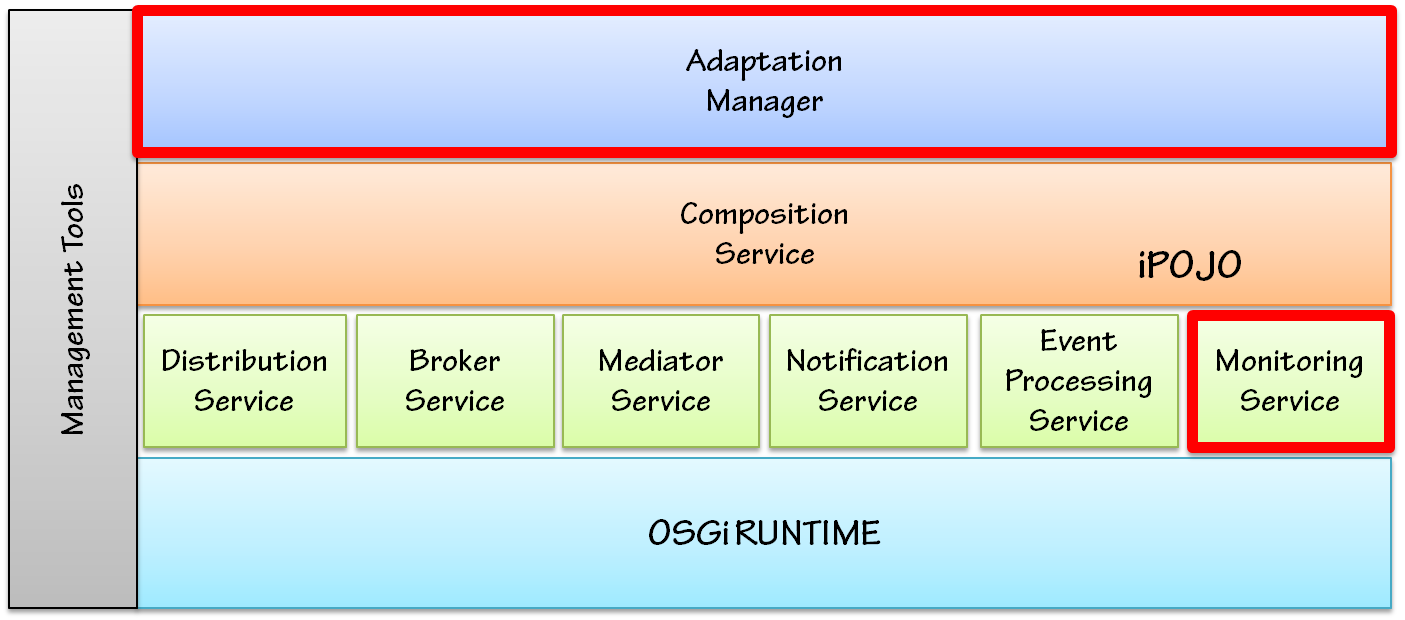
\includegraphics[width=13cm]{chapters/chapter4/dsoa-provider-manager.png}
\caption[Visão Geral da Proposta na Arquitetura]{Visão Geral da Proposta na Arquitetura.}
\label{fig:proposal}
\end{figure}

A combinação destes 2 módulos, junto aos serviços providos pela plataforma surge como uma solução para o problema de gestão de provedores de servico. Detalhadaremos seu funcionamento e arquitetura nas próximas seções.

\section{Arquitetura}
%TODO explicar arquitetura


\subsection{Módulo de Monitoração de Recursos}
%TODO: definir módulo

Os dados do monitoramento são enviados, através da figura de eventos, ao serviço de processamento de eventos que gera notificações ao gerenciador do provedor de serviços quando algum problema é detectado.%[FIXME: como explicar isso ¬¬] 

\begin{figure}[htp]
\centering
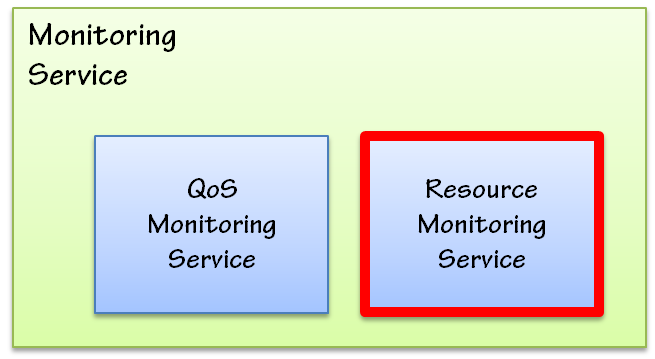
\includegraphics[width=9cm]{chapters/chapter4/monitoring-service.png}
\caption[Resource Monitoring Service]{Resource Monitoring Service.}
\label{fig:resc_module}
\end{figure}


\subsection{Módulo de Gerencimento de Provedor}
%TODO: definir módulo

\begin{figure}[htp]
\centering
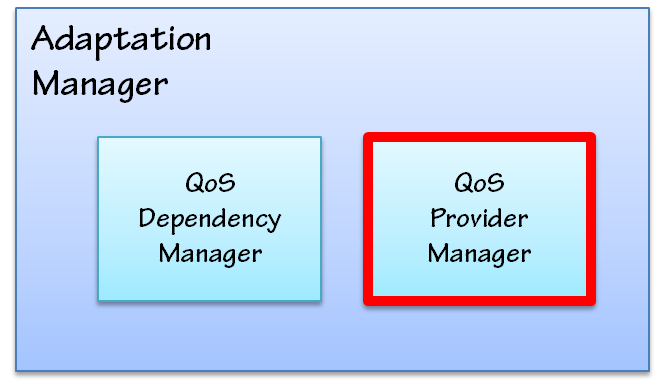
\includegraphics[width=9cm]{chapters/chapter4/adaptation-manager.png}
\caption[QoS Provider Manager]{QoS Provider Manager.}
\label{fig:proposal}
\end{figure}


\section{Aplicação do Ciclo PDCA}
Todo o processo de monitoramento e adaptação será baseado nas etapas definidas pelo ciclo PDCA.

Como vimos na Seção \ref{sec:pdca}, o ciclo foca em manter ou melhorar a qualidade de processos, com base nas informações referentes a sua execução.

\begin{figure}[htp]
\centering
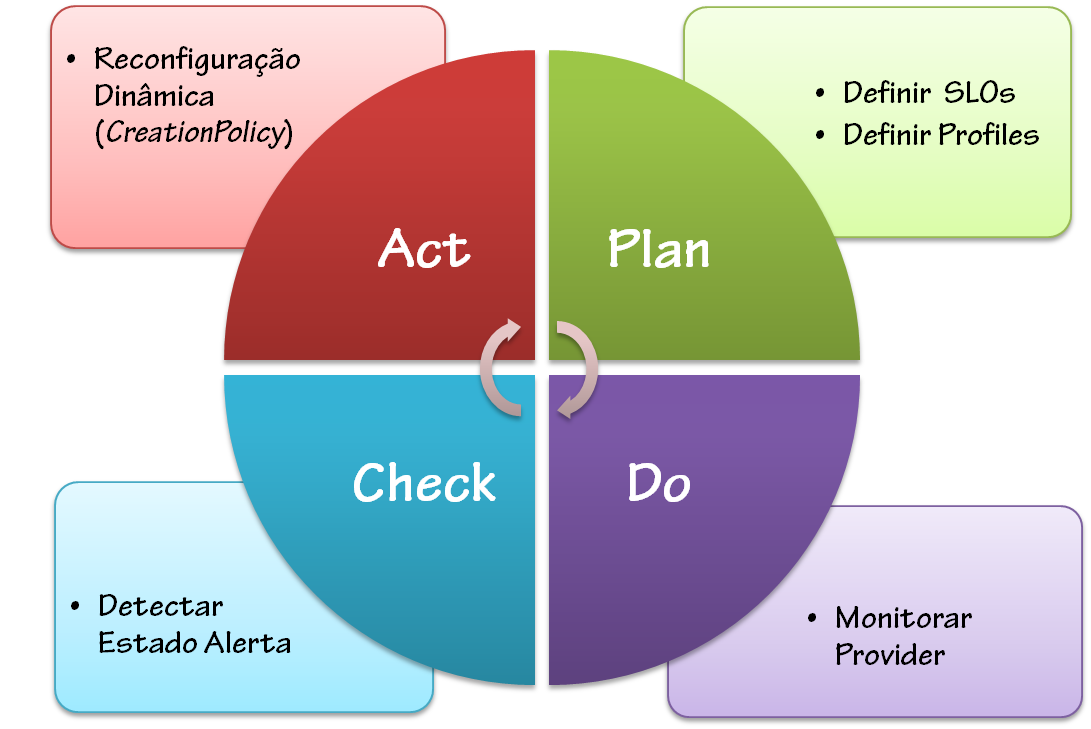
\includegraphics[width=10cm]{chapters/chapter4/pdca_actions.png}
\caption[Aplicação do Ciclo PDCA]{Aplicação do Ciclo PDCA.}
\label{fig:pdcamapping}
\end{figure}


Na etapa de planejamento, as metas serão definidas por meio de um documento XML~\cite{xml} que descreve as capacidades que o provedor afirma garantir. Essas propriedades são utilizadas para definir configurações de monitoração (\textit{Monitoring Configuration}) relacionadas a atributos de qualidade do provedor (\textit{e.g} tempo de processamento).

Essas metas são definidas através da \textit{tag} \verb slo , que descreve uma métrica a ser medida, um valor de \textit{threshold} e uma relação de limite(máximo ou mínimo) que o valor do \textit{threshold} pode ultrapassar. Em alguns casos, temos também o indentificador da operação provida. Essa informação é útil em casos de configurações de monitoração relacionadas a invocações de determinados métodos do provedor (e.g. \textit{throuhput} de uma operação). Ver Apêndice \ref{subsec:slo}.

Além disso, também são definidos no mesmo XML, métodos que visam sanar possíveis causas que impactem no desempenho do provedor, buscando garantir que as capacidades apresentadas sejam devidamente providas.

Esses métodos são descritos pela \textit{tag} \verb profile , que define um conjunto de \verb profiles ~que relacionam configurações de monitoração a políticas de gerenciamento de instâncias, que visam evitar a degradação do sistema. 

Um \textit{profile} especificar um conjunto de \verb resources , semelhantes aos \textit{slos}, com o objetivos de definir uma configuração de monitoração


\begin{figure}[htp]
\centering
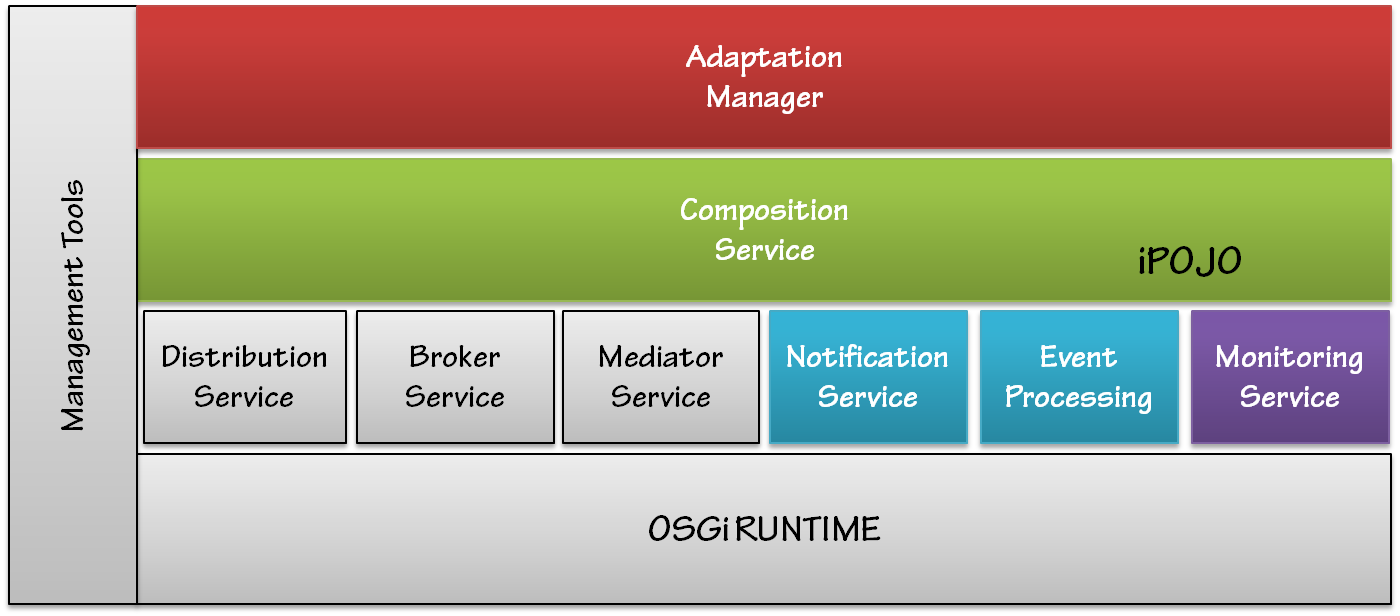
\includegraphics[width=13cm]{chapters/chapter4/pdca_arch_overview.png}
\caption[Componentes da Arquitetura x Fases PDCA]{Componentes da Arquitetura x Fases PDCA.}
\end{figure}
